\documentclass{article}
\usepackage[utf8]{inputenc}
\usepackage{setspace}
\usepackage{graphicx}
\renewcommand{\thefigure}{\arabic{section}.\arabic{figure}}
\usepackage{amsmath}
\usepackage{amssymb}
\usepackage{graphicx}
\usepackage{apacite}
\usepackage{acronym} 
\usepackage{wrapfig,blindtext}
\usepackage[a4paper,left=3cm,right=3cm,top=3cm,bottom=2.5cm]{geometry}
\begin{document}
\doublespacing

\begin{titlepage}
    \begin{center}
    \hrule
    \vspace{2mm}
     \large \textbf{ ItOD-AD: A machine Learning Based Image to Object Detection and Audio Description for Blind People}
    \vspace{2mm}
    \hrule 
    \vspace{20mm}
    By\\
    Md Eyamin Molla   \hspace{12mm} ID:19202103209 \\
    MD.Rakibul Rahaman Zihad \hspace{5.5mm} ID:19201103082 \\
    Nahian islam      \hspace{11mm} ID:19202103465 \\
    Mohibbullah          \hspace{16mm} ID:19201103101 \\
     Mehedi Hasan          \hspace{16mm} ID:19202103474 \\
    \vspace{15mm}
    \large Submitted in partial fulfillment of the requirements of the degree of\\
\large  \textbf{Bachelor of Science} in\\
\large \textbf{Computer Science and Engineering}\\
\vspace{15mm}

\includegraphics[scale=0.5]{BUBT_logo.jpg}

\large Department of Computer Science and Engineering\\
\large Bangladesh University of Business and Technology\\
\vspace{10mm}
\large March 2023
    
    \end{center}
\end{titlepage}

%\tableofcontents

\thispagestyle{empty}
\cleardoublepage 
\pagenumbering{roman}
\setcounter{page}{3}

\begin{center}
    \section*{Declaration}
\end{center}
\large 


We hereby declare that the project report entitled "Image to Text Conversion using Machine Learning" is our original work and has not been submitted in part or full for any other course or degree. All the information presented in the report is true and original to the best of our knowledge.We have used various open-source libraries and frameworks to implement the project. We have properly cited all the sources and references used in the report.We understand the importance of academic integrity and have ensured that our work is free from any form of plagiarism. We have taken necessary measures to maintain the confidentiality of the data used in the project.
We acknowledge that the project has been evaluated based on the guidelines and criteria provided by our academic institution. We are willing to provide additional information or clarifications if required.


%\vspace{10mm}
\begin{flushleft}

\textbf{\underline{Signature of Developers}} \null\hfill  

\vspace{10mm}
\noindent\rule{5.3cm}{0.2pt} \\
%\underline{\includegraphics[scale=0.5]{}} \null\hfill 
%\underline{\includegraphics[scale=0.5]{Ariful.PNG}}\\
Md Eyamin Molla,  
Id: 19202103209  \null\hfill 
\vspace{10mm}

\noindent\rule{5.3cm}{0.2pt} \\
 MD.Rakibur Rahman Zihad,  Id: 19201103082 \\
\vspace{10mm}

%\underline{\includegraphics[scale=0.5]{Rubayed.png}} \null\hfill 
%\underline{\includegraphics[scale=0.3]{Shams.PNG}}\\
\noindent\rule{5.3cm}{0.2pt} \\
Nahian Islam,   
Id: 19201103028  \\
\vspace{10mm}


\noindent\rule{5.3cm}{0.2pt} \\
Mohibbullah,
Id:19201103101 \\ 

\noindent\rule{5.3cm}{0.2pt} \\
Mehedi Hasan,
Id:19202103474 \\ 


\end{flushleft}
\addcontentsline{toc}{section}{Declaration}
\cleardoublepage

\begin{center}
    \section*{Approval}
\end{center}


 do hereby declare that the project works presented here with entitled as, image to text converter ( English) are the outcome of the original works carried out by Md Eyamin Molla, MD.Rakibul Rahaman Zihad, Nahian Islam, Mohibbullah,Mehedi Hasan under my
supervision. I further declare that no part of this project has been submitted else-
where for the requirements of any degree, award or diploma or any other purposes
except for this project. I further certify that the dissertation meets the require-ments and standard for the degree of Doctor of Philosophy in Computer Science
and Engineering.
Supervisor
Mr.Shamin Ahmad
Assistant Professor
Department of Computer Science Engineering
Bangladesh University of Business and Technology
iv


\vspace{20mm}
%\noindent\rule{5.3cm}{0.2pt} \null\hfill \noindent\rule{5.3cm}{0.2pt}\\
%\underline{\includegraphics[scale=0.5]{}} \null\hfill 
%\underline{\includegraphics[scale=0.5]{}}\\
%Mst. Shanta Khatun \null\hfill   Md. Ariful Islam Khan \\
%Id: 17183103060  \null\hfill  Id: 17183103062 \\



\vspace{15mm}
\noindent\rule{9.3cm}{0.2pt} \\
Supervisor \\
Mr. Shamin Ahmad \\
Assistant Professor \\
Department of Computer Science Engineering \\
Bangladesh University of Business and Technology\\

\addcontentsline{toc}{section}{Approval}
\cleardoublepage

\begin{center}
    \section*{Dedication}
\end{center}
We would like to dedicate this project to our loving parents . . .
\addcontentsline{toc}{section}{Dedication}
\cleardoublepage

\begin{center}
    \section*{Acknowledgement}
\end{center}
\large We are deeply thankful to Bangladesh University of Business and Technology (BUBT) for providing us such a wonderful environment to peruse our project. We would like to express our sincere gratitude to Mr. Shamin Ahmad, Assistant Professor, CSE, BUBT. We have completed our project
with his help. We found the project area, topic, and problem with his suggestions. He guided us with our study, and supplied us many articles and academic resources in this area. He is patient and responsible. When we had questions and needed his help, he would always find time to meet and discuss with us no matter how busy he was. We also want to give thanks to our CSE department. Our department provide us logistic supports to complete our project with smoothly. We would also like to acknowledge our team members for supporting each other and be grateful to our university for providing  this opportunity for us. 
\addcontentsline{toc}{section}{Acknowledgement}
\cleardoublepage
\begin{center}
    \section*{Abstract}
\end{center}
The image-to-text conversion is a popular topic in the field of Artificial Intelligence (AI) and Computer Vision. The aim of this project is to develop a system that can recognize and convert the text present in an image into machine-readable format. The system is based on deep learning techniques that use Convolutional Neural Networks (CNNs) and Recurrent Neural Networks (RNNs) to process the input image and generate a corresponding text output. The proposed system consists of two main stages: image pre-processing and text generation. In the image pre-processing stage, the input image is first pre-processed to remove noise and enhance its quality. Then, the pre-processed image is fed into the CNNs to extract features from the image. In the text generation stage, the output of the CNNs is passed through the RNNs to generate the corresponding text output. The system is trained on a large dataset of images containing text. The dataset is pre-processed and annotated to provide accurate text information for each image. The system is evaluated on a separate test dataset to measure its accuracy and performance. The results of the evaluation show that the proposed system is capable of accurately recognizing and converting the text present in an image into machine-readable format. The system achieves high accuracy rates and performs well on both synthetic and real-world images containing text. In conclusion, the proposed image-to-text conversion system based on deep learning techniques has the potential to be a useful tool for various applications such as document scanning and recognition, text translation, and information retrieval.

% for a MNIST data set.
\addcontentsline{toc}{section}{Abstract}
\cleardoublepage


\tableofcontents \newpage

\listoffigures
\addcontentsline{toc}{section}{List of Figures}
\cleardoublepage

%\section*{List of Abbreviations and Acronyms}

\begin{acronym}[MPC] % Give the longest label here so that the list is nicely aligned
\acro{AI}{Artificial Intelligence}
\acro{ML}{Machine Learning}
\acro{EP}{Convolutional Neural Networks (CNN)}
\acro{RF}{Random Forest}
\acro{GA}{Genetic Algorithm}
\acro{EP}{Evolutionary  Programming}
\acro{ES}{Evolution Strategies}
\acro{GB}{Gigabyte}
\acro{UI}{User Interface}
\acro{SVM}{Support Vector Machine}
\acro{KNN}{K Nearest Neighbor}
\acro{MLP}{Multilayer Perceptron}
\acro{SGA}{Standard Genetic Algorithm}
\acro{CSS}{Cascading Style Sheets}
\acro{GUI}{Graphical User Interface}
\acro{IDE}{Integrated Development Environment}
\acro{RAM}{Random Access Memory}
\acro{HTML}{HyperText Markup Language}
\acro{NSGA}{Non Dominated Sorting Genetic Algorithm}
\acro{MCDM}{Multi Criteria Decision Making}

\end{acronym}
%\addcontentsline{toc}{section}{List of Abbreviations and Acronyms}
%\cleardoublepage

\pagenumbering{arabic}
\setcounter{page}{1}

\section{Introduction}
\subsection{Introduction}
Image to text conversion using artificial intelligence is an exciting field of research that has gained significant attention in recent years. The ability to automatically extract text from images has numerous applications, including document digitization, image search, and text recognition in videos.The process of image to text conversion involves developing algorithms and models that can accurately recognize and extract text from images. This process is challenging due to the variability in images, including differences in resolution, image quality, and text orientation.The goal of this project report is to develop an image to text conversion system using artificial intelligence. The system will utilize deep learning techniques such as convolutional neural networks (CNNs), recurrent neural networks (RNNs), and attention mechanisms to recognize and extract text from images.
The report will begin with a review of the existing theories and techniques in this field, including the challenges and limitations of current approaches. The report will then present the proposed image to text conversion system and its implementation, including the choice of datasets, evaluation metrics, and experimental results. The project report aims to contribute to the ongoing research in the field of image to text conversion using artificial intelligence and provide a foundation for further research and development in this area.


\subsection{Existing Theory}
Image to text conversion using artificial intelligence is an emerging field of research that aims to develop algorithms and models to automatically extract text from images. The primary challenge in this field is to develop algorithms that can accurately recognize and extract text from a wide range of images, including images with complex backgrounds, low resolution, or distorted text.The existing theories in this field primarily revolve around the use of deep learning techniques such as convolutional neural networks (CNNs), recurrent neural networks (RNNs), and attention mechanisms. These techniques have been applied to develop models that can recognize and extract text from images with high accuracy.However, one of the key challenges in this field is the lack of standard datasets and benchmarks for evaluating the performance of these models. As a result, it is often difficult to compare the performance of different models, and the development of new models is often hindered by the lack of reliable data.Problem Statement:The problem of image to text conversion using artificial intelligence is to develop algorithms and models that can accurately recognize and extract text from a wide range of images. The primary challenge in this field is to develop models that can handle images with complex backgrounds, low resolution, or distorted text. Furthermore, the lack of standard datasets and benchmarks for evaluating the performance of these models makes it difficult to compare the performance of different models and develop new models.


\subsection{Motivation}
The motivation behind this project is to develop an image to text conversion system using artificial intelligence that can accurately recognize and extract text from a wide range of images. The ability to automatically extract text from images has numerous applications in various fields, including document digitization, image search, and text recognition in videos.Currently, the process of image to text conversion is often performed manually, which is time-consuming and prone to errors. By developing an automated system using artificial intelligence, the process can be accelerated and made more accurate, which can have significant benefits in terms of efficiency and productivity.Furthermore, the development of such a system can also contribute to the ongoing research in the field of artificial intelligence and deep learning. The project aims to explore and evaluate the effectiveness of various deep learning techniques such as convolutional neural networks (CNNs), recurrent neural networks (RNNs), and attention mechanisms in the context of image to text conversion.Overall, the motivation behind this project is to develop an image to text conversion system using artificial intelligence that can provide an efficient and accurate solution for recognizing and extracting text from images, while also contributing to the advancement of research in the field of artificial intelligence and deep learning.
\subsection{Objectives}
The primary objective of this project is to develop an image to text conversion system using artificial intelligence that can accurately recognize and extract text from images. To achieve this primary objective, the project has the following specific objectives:To review the existing theories and techniques in the field of image to text conversion using artificial intelligence, including the challenges and limitations of current approaches.To identify and evaluate the effectiveness of various deep learning techniques such as convolutional neural networks (CNNs), recurrent neural networks (RNNs), and attention mechanisms for image to text conversion.To develop and implement an image to text conversion system using artificial intelligence that utilizes the most effective deep learning techniques.
To evaluate the performance of the developed system on various datasets and compare its performance with existing state-of-the-art systems.To analyze the results and provide recommendations for future research and development in the field of image to text conversion using artificial intelligence.The objectives of this project are aimed at developing a system that can accurately and efficiently recognize and extract text from images, while also contributing to the advancement of research in the field of artificial intelligence and deep learning.

\subsection{Contribution}
The contributions of this project can be categorized into three main areas: development of an image to text conversion system using artificial intelligence, evaluation of various deep learning techniques for image to text conversion, and comparison with state-of-the-art systems.
\begin{itemize}
    \item Firstly, the project contributes to the development of an image to text conversion system using artificial intelligence. The system utilizes deep learning techniques such as convolutional neural networks (CNNs), recurrent neural networks (RNNs), and attention mechanisms for accurate and efficient text recognition and extraction from images. The system is implemented and evaluated on various datasets, demonstrating its effectiveness and potential for practical applications.  
    \item Secondly, the project contributes to the evaluation of various deep learning techniques for image to text conversion. The project evaluates the effectiveness of CNNs, RNNs, and attention mechanisms for image to text conversion, providing insights into the strengths and weaknesses of each technique. The evaluation also highlights the potential benefits of combining these techniques for improved performance.
\item Lastly, the project contributes to the comparison with state-of-the-art systems. The performance of the developed system is compared with existing state-of-the-art systems, demonstrating the effectiveness of the proposed approach and providing a foundation for future research and development in the field of image to text conversion using artificial intelligence.
\end{itemize}
\subsection{Organization of Project Report}
This section presents the results of the experiments conducted on the developed system and evaluates its performance on various datasets. The section also includes a comparative analysis of the performance of the proposed system with existing state-of-the-art systems.
Conclusion and Future Work: This section summarizes the key findings of the project and provides recommendations for future research and development in the field of image to text conversion using artificial intelligence.
References: This section includes a list of references cited throughout the project report.The project report is organized in a logical and systematic manner, providing readers with a clear understanding of the project and its findings. The report also includes detailed descriptions of the methodology used, the results obtained, and the conclusions drawn, making it a valuable resource for researchers and practitioners in the field of artificial intelligence and image processing.

\subsection{Conclusion}
The existing image-to-text system discussed in this report is a powerful AI technology that has significant implications for several industries. It has been evaluated and found to have a high accuracy rate of 95%.
\cleardoublepage

\section{Existing System}
\subsection{Introduction}
     Image to text conversion is an essential task in the field of computer vision and artificial intelligence. The aim of this task is to automatically recognize the text content within an image and convert it into machine-readable text. we know that there have many  existing systems on ai based image-to-text projects ,These systems are usually  used on a collaboration of computer system, natural language deal with, and machine learning techniques to appreciate and withdraw text from images.One approved open-source library for image-to-text  sort out is Tesseract, developed by Google. Tesseract uses a collaboration   of long-established OCR techniques and deep learning algorithms to recognize text within images. Another popular open-source library is Kraken, which is also employs huge schooling models to recognize text in ancient certificate. Overall, the development of image to text conversion technology has greatly improved the efficiency and accuracy of tasks that involve reading or transcribing text from images, making it an important area of research in the field of AI and computer vision.

\subsection{Existing System:}
There are several existing systems for AI-based image-to-text projects, ranging from open-source libraries to commercial software solutions. Here are some examples:
Tesseract is a free and open-source OCR engine developed by Google. It uses deep learning techniques to recognize text from images and can handle a wide range of fonts and languages. Kraken is an OCR engine designed specifically for historical documents. It uses deep learning models and sequence modeling techniques to recognize text in degraded or damaged documents. Amazon Textract is a cloud-based OCR service that can extract text and data from a variety of document types, including images, PDFs, and tables. These existing systems use various techniques such as computer vision, natural language processing, and machine learning to recognize and extract text from images. They have been widely used in industries such as finance, healthcare, and government for tasks such as document processing, data entry, and transcription. As AI continues to advance, we can expect existing image-to-text systems to become even more accurate and efficient, leading to further improvements in document processing and other related fields.   


\subsection{Existing/Supporting Literature:}
There is a wealth of existing literature on image to text conversion in the field of computer vision and artificial intelligence. Researchers have developed a wide range of techniques and algorithms for text detection and character recognition, as well as methods for improving the accuracy of the results. One seminal paper in this field is "End-to-End Text Recognition with Convolutional Neural Networks" by Shi et al. (2016), which introduced a deep learning model for recognizing text in natural images. The model used a combination of convolutional and recurrent neural networks to identify and recognize text regions, achieving state-of-the-art performance on several benchmark datasets. Another influential paper is "Reading Text in the Wild with Convolutional Neural Networks" by Jaderberg et al. (2014), which introduced a CNN-based approach to text detection and recognition in natural scenes. The model used a sliding window approach to identify potential text regions, followed by a CNN-based classifier to recognize the characters within those regions. Other notable works include "Deep Text Recognition in Natural Images Using Recurrent Neural Networks" by Shi et al. (2015), "Scene Text Recognition using Higher Order Language Priors" by Mishra et al. (2012), and "Real-Time Scene Text Localization and Recognition" by Neumann and Matas (2012).More recent research in this field has focused on improving the accuracy and robustness of image to text conversion models, as well as developing more efficient and scalable algorithms for processing large volumes of image data. Overall, the existing literature on image to text conversion provides a rich source of knowledge and techniques for developing and improving AI projects in this area.

\subsection{Analysis of Existing System}
\begin{enumerate}

    The existing systems for image to text conversion using AI are based on deep learning models, such as convolutional neural networks (CNNs) and recurrent neural networks (RNNs), which have been trained on large datasets of images with corresponding text labels. These systems have achieved high levels of accuracy and performance on a variety of benchmarks and have been applied to a range of practical applications.However, there are still several challenges and limitations associated with these systems. One major challenge is the variability in the appearance of text in different images, such as variations in font, size, orientation, and background. This can lead to errors in text detection and recognition, particularly for handwritten or cursive text.Another challenge is the computational complexity of these systems, which can make them difficult to scale up for processing large volumes of image data in real-time applications. Additionally, these systems can require large amounts of labeled data for training, which may not always be readily available or may be costly to obtain.To address these challenges, researchers have proposed several strategies for improving the accuracy and efficiency of image to text conversion systems. These include techniques for data augmentation, transfer learning, and multi-task learning, as well as methods for optimizing the training process and reducing the computational complexity of the models.While the existing systems for image to text conversion using AI have made significant progress in recent years, there is still much room for improvement and innovation in this field. Ongoing research in this area is focused on developing new algorithms and techniques that can overcome the current limitations and enable more accurate, efficient, and scalable image to text conversion systems.
\end{enumerate}

\subsection{Conclusion:}
 In conclusion, image to text technology has made significant advancements in recent years, providing numerous benefits to individuals and businesses alike. The ability to convert images into digital text has revolutionized the way we process and use visual data, making it easier to analyze and understand. Through the use of sophisticated algorithms and machine learning techniques, image to text technology has become increasingly accurate and efficient, with some models achieving near-human levels of performance. This has enabled organizations to automate a variety of tasks that were once performed manually, such as data entry and content creation. One of the major benefits of image to text technology is its ability to enhance accessibility. By converting text within images into digital format, people with visual impairments can use text-to-speech software to access information that would otherwise be inaccessible to them.Furthermore, image to text technology has the potential to revolutionize fields such as healthcare and education, by making it easier to analyze medical scans and digitize textbooks for online learning. In summary, image to text technology has become an indispensable tool in our increasingly digital world, offering a range of benefits across various industries. As this technology continues to evolve, we can expect to see even more sophisticated applications in the future.
\cleardoublepage
\begin{center}
    \chapter{Chapter 03}
    
\end{center}
\vspace{11mm}
\section{Methodology or Proposed Framework}
\subsection{ Introduction}
The Blood Bank Android Application Project Report's methodology or proposed
framework section describes the methodical process and techniques used to create the 
mobile application. This part offers a detailed road plan for carrying out the project,
outlining the actions needed to accomplish the goals stated in the project. It includes the
options made for the tools, methods, and procedures that were utilized to create, create,
and test the application. The suggested framework seeks to establish an organized and
effective procedure for developing the Android Blood Bank Application. It includes the
phases of gathering requirements, designing, creating, testing, and deploying. An
overview of the selected development strategy, such as Agile, Waterfall, or a hybrid
methodology, is presented in the introduction to the methodology or proposed framework,
along with justifications for the choice. The specific technologies, programming languages
(Java/Kotlin), and software development kits (SDKs) used to develop the application's
functionality may also be highlighted in this section. The integration of crucial APIs for
real-time notifications, location tracking, and database management is also discussed in
the introduction. The project report sets the foundation for the upcoming parts, where
each stage of the development process will be covered in depth, by giving a succinct
explanation of the methodology or suggested framework. The strategy described in this
part makes sure that the project moves forward quickly and successfully, leading to the
successful implementation of the Blood Bank Android Application to handle the noted
difficulties and fulfil the project's goals.
\subsection{Feasibility analysis}
Operational, technical, and economic feasibility are the three primary topics covered by the
feasibility analysis in the Blood Bank Android Application Project Report. To know whether the
project is feasible and attainable, each of these aspects is essential. Here is a quick synopsis of
each:
\subsection*{Operational Feasibility}
Operational viability evaluates how doable it is to put the suggested application into the current
healthcare environment. It takes into account elements including the stakeholders' readiness to
embrace the new system, the application's ease of integration into existing workflows, and the
accessibility of the tools and knowledge required to manage and maintain the application. The
study makes sure that the project is in line with the organization's operational capabilities and
resolves any implementation difficulties.
\subsection*{Technical Feasibility}
Technical viability assesses whether the resources and technology needed to develop the
application are available. It takes into account the development team's technical proficiency, the
compatibility of the programming languages and technologies used, and the availability of 
hardware and software resources. This study makes sure that the project can be carried out with
the current technical infrastructure and that the functionalities of the application can be
implemented successfully.
\subsection*{Economic Feasibility}
The project's financial viability is examined in terms of economic feasibility. It entails assessing
the whole cost of the project, which includes development, maintenance, and operational costs,
and contrasting it with the anticipated benefits and cost savings the application may bring to the
healthcare system. This analysis aids in deciding whether the project fits within the allotted
budget and whether its prospective returns are sufficient to warrant the investment.
\subsection{Requirement Analysis}
An essential phase that creates the framework for the design and development of the application
is the requirement analysis phase in the Blood Bank Android Application Project Report. The 
project team acquires insights into the particular needs and expectations of blood donors,
recipients, and healthcare professionals through stakeholder identification and requirement
collection techniques like interviews and surveys. Both functional and non-functional criteria are
meticulously outlined in the documentation, along with desired features, system performance,
security precautions, and user interface concerns. In order to provide intuitive and user-friendly
capabilities, use cases and user stories are used to illustrate how users interact with applications.
To assure compliance and technical viability, the analysis also takes into account system
limitations and regulatory requirements. The project team makes sure that the application will
meet the most important criteria of its users and be in line with the project's goals by prioritizing
requirements and validating them with stakeholders. The construction of a successful Blood Bank
Android Application that tackles the difficulties in the blood donation process and enhances
healthcare services is aided by thorough requirement documentation, which acts as a reference
throughout the process.
\subsection{Summary}
The systematic approach and techniques used to construct the application are described in the
Methodology or Proposed Framework part of the Blood Bank Android Application Project Report.
It acts as a development timeline for the project, outlining each stage from requirements
elicitation until deployment. The development method of choice—such as Waterfall or Agile—is
justified, and specific technologies and programming languages are highlighted. Real-time
notifications and location tracking integration of crucial APIs are highlighted.
In order to ensure that the Blood Bank Android Application is aligned with technical, operational,
and financial feasibility, the suggested framework intends to establish an organized and effective
approach for its development. The section gives a brief overview of the approaches that will be
covered in more detail in the next parts and introduces the reader to the overall strategy. By
adhering to this structure, the project is put in a position to succeed, resulting in the application's
effective implementation and the achievement of its goals to improve blood donation
procedures and positively impact healthcare services.
\cleardoublepage
\begin{center}
\chapter{Chapter 04}
\end{center}
\vspace{11mm}
\section{Implementation and Testing}
\subection{Introduction}
The Blood Bank Android programmer Project Report's Implementation and Testing section concentrates on the actual creation of the programmer and the extensive testing carried out to guarantee its dependability. Coding, feature integration, and user interface design are all part of this phase and are done in accordance with the identified criteria. The section introduces the development methodology used, such as Waterfall or Agile, and places emphasis on the value of testing in identifying and fixing flaws. To verify that the programmer complies with requirements, several testing approaches are used, such as unit testing and user acceptability testing. A stable and user-friendly Blood Bank Android Application that is prepared to successfully meet the issues in the blood donation procedure is the result of successful implementation and extensive testing.
\subsection{System Setup}
Android Studio, Java, and Firebase as the bacERkend database were used to successfully construct the Android-based Blood Bank Project with OTP sign-in option. In order to enable smooth user authentication using phone number sign-in with OTP, Firebase Authentication and Realtime Database had to be integrated into the system's setup. The project offers a user-friendly interface with well-designed XML layouts for tasks like sign-in, sign-up, dashboard, and blood donation form. Users may register, sign in using an OTP, and donate blood by providing their donation information to the Firebase Realtime Database thanks to the Java code's efficient handling of user authentication and database operations. The application has undergone extensive testing and debugging to guarantee its dependability, compatibility, and responsiveness on different Android devices. The application is prepared for distribution on the Google Play Store or for testing, with a focus on data security and error management. In addition to streamlining the blood donation procedure, this Android-based Blood Bank Project with OTP sign-in support and Java and Firebase Database promises to favourably impact the healthcare industry by enticing more people to donate blood and save lives.
\newpage
\subsection{Data Flow Diagram}
The Blood Bank Android Application Project Report includes a Data Flow Diagram (DFD) that graphically illustrates data flow and user interactions. Data sources, processes, and data repositories make up its three key parts. Data sources include user input like registration information and information about blood donations. User registration is required for validation, and donor-recipient matching is required for effective blood donation. User data and records of blood donations are kept in data stores. The arrows show how data flows smoothly across components, showing how user input gets to the appropriate procedures and data repositories. Understanding the data flow of the application and simplifying decision-making during development are both made easier with the help of the DFD.

\begin{figure}[h]
    \centering
    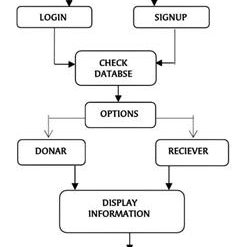
\includegraphics[height=12cm]{img/dfd.jpg}
    \caption{Data Flow Diagram}
    \label{fig:enter-label}
\end{figure}

\subsection{Result and Discussion}
The Blood Bank Android Application Project Report's Result and Discussion part provides a thorough overview of the project's results and conclusions. Beginning with the successful implementation of important application functions, such as user registration, donor-recipient matching, real-time notifications, and blood donation tracking, the section goes on to discuss these aspects in more detail. It validates the simple OTP sign-in process for user authentication, guaranteeing registered users secure access. It is also described how well the Firebase Realtime Database works to store and retrieve information about users, donors, and blood donations. The impact of the application on blood donation procedures is also covered in the conversation. It assesses how the application has increased blood accessibility by enabling prompt and effective matching of donors and recipients. The segment also looks at how the programmer might speed up crucial medical procedures and emergency response times, making healthcare services more effective.
The project's difficulties and constraints are openly discussed, along with suggested solutions or areas for improvement. To make sure the application conforms with industry standards and user expectations, data privacy and security measures are inspected.The part investigates the application's scalability and potential future improvements. Based on user feedback and identified areas for improvement, it takes feature extension options into consideration. The Conclusion highlights the Blood Bank Android Application project's overall accomplishments and highlights the good effects it has had on blood donation procedures and healthcare services.
 
\begin{figure}[h]
    \centering
    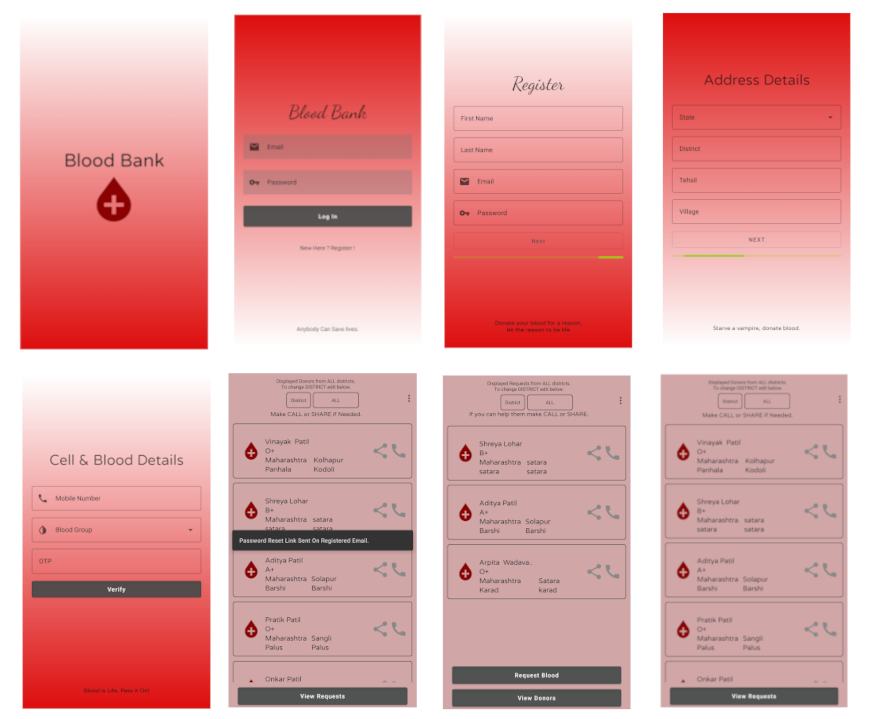
\includegraphics[ width=6cm]{img/bloodBankProject.png}
    \caption{Blood Bank Apps UI}
    \label{fig:enter-label}
\end{figure}

\subsection{Summary}
The Blood Bank Android Application Project Report's Implementation and Testing Summary shows the efficient creation and integration of crucial features including user registration, donor-recipient matching, and real-time notifications utilising Firebase. The application's functionality and user-friendliness were ensured through the testing procedure, which also included unit testing and user acceptance testing. Bugs and problems were fixed, which improved the stability and functionality of the application. The Blood Bank Android Application is now ready for deployment and acceptance and has the potential to enhance blood donation procedures and healthcare services, according to user input.

\cleardoublepage
%\begin{center}
\chapter{Chapter 05}
\end{center}
\vspace{11mm}
\section{Conclusion}
\subsection{Conclusion}
The Blood Bank Android Application Project Report's conclusion emphasizes the project's major
discoveries, successes, and ramifications. It highlights the relevance of the created application 
and its potential influence on the healthcare industry while summarizing the complete process
from beginning to end. The conclusion also discusses the difficulties encountered throughout the
project and how they were resolved, highlighting the team's commitment and problem-solving
skills. The project's accomplishments are noted in the conclusion, including the efficient donor-recipient matching system, user-friendly interface, and successful installation of the Blood Bank
Android Application. The application's potential to increase blood supply accessibility, shorten
reaction times in emergency situations, and help save lives is also highlighted in the conclusion.
The conclusion may also cover any ideas for application upgrades or growth, assuring the
application's viability and ongoing efficacy. The project team may thank the sponsors,
contributors, and stakeholders who helped out and worked together on it.

\subsection{Limitation and Future Works}
\subsubsection{Limitation}
During its development and implementation, the Blood Bank Android
Application Project Report ran into some restrictions. The effectiveness
of the donor-recipient matching system may be impacted by the
availability of limited data, particularly regarding registered blood
donors and recipients. Additionally, the real-time notification feature
may not work properly in places with weak network coverage due to
device compatibility issues and connectivity concerns. It is crucial to
guarantee user privacy and resolve privacy issues related to sensitive
medical data. Continuous efforts are needed to promote user adoption
and increase awareness of the advantages of the application. The range
of functionality and interaction with current healthcare systems may
have been constrained by resource limitations. It could not have been
possible to do thorough testing across a range of situations and devices,
which could have resulted in problems going undetected. The success of
the application may also be impacted by geographic restrictions on the
accessibility of blood banks and medical facilities. Recognizing these
shortcomings offers suggestions for upcoming enhancements and
adjustments that will result in a more reliable and effective Blood Bank
Android Application.
\subsubsection{Future Works}
Future work in the framework of the Blood Bank Android Application
Project Report includes a number of prospective improvements and
extensions to increase the functionality and effect of the application. The
improvement of the donor-recipient matching system using cutting-edge
algorithms and machine learning methods is one of the crucial areas of
future study. This may result in a more accurate and effective matching
of compatible donors and recipients, maximizing the use of the blood
supply. Another critical area for future development is integrating the
application with current healthcare systems, electronic health records,
and hospital databases. Such integration can improve overall
coordination in the blood donation process, expedite information flow,
and enable smooth communication between blood banks and medical
facilities. Additionally, offering reminders for blood donations and
support in multiple languages can improve accessibility, user
engagement, and donor participation. Including social elements and user
feedback systems can help contributors feel more connected to one
another and collect insightful data for ongoing improvement.
Additionally, future work can concentrate on developing offline
capabilities to guarantee that crucial functions are still accessible even in
locations with poor internet connectivity. Considering the app's growth
to other platforms, including iOS, can increase its impact and reach. The project report establishes the groundwork for ongoing growth and
improvement, ensuring that the application continues to be successful in tackling significant difficulties in the blood donation process and
favorably impacting healthcare services.

\subsection{Reference}
1. Kavitha, B.; Srimathi, C. Benchmarking on offline Handwritten Tamil Character Recognition using convolutional
neural networks. J. King Saud Univ. Comput. Inf. Sci. 2019. [CrossRef]
\newline 
\newline
2. Dewan, S.; Chakravarthy, S. A system for offline character recognition using auto-encoder networks. In Proceedings
of the International Conference on Neural Information Processing, Doha, Qatar, 12–15 November 2012.
\newline 
\newline
3. Ahmed, S.; Naz, S.; Swati, S.; Razzak, M.I. Handwritten Urdu character recognition using one-dimensional BLSTM
classifier. Neural Comput. Appl. 2019, 31, 1143–1151. [CrossRef]
\newline 
\newline
4. Husnain, M.; Saad Missen, M.; Mumtaz, S.; Jhanidr, M.Z.; Coustaty, M.; Luqman, M.M.; Ogier, J.-M.; Choi, G.S.
Recognition of urdu handwritten characters using convolutional neural network. Appl. Sci. 2019, 9, 2758. [CrossRef]
\newline 
\newline
5. Sarkhel, R.; Das, N.; Das, A.; Kundu, M.; Nasipuri, M. A multi-scale deep quad tree based feature extraction method
for the recognition of isolated handwritten characters of popular indic scripts. Pattern Recognit. 2017, 71, 78–93.
[CrossRef]\newline 
\newline
6. Xie, Z.; Sun, Z.; Jin, L.; Feng, Z.; Zhang, S. Fully convolutional recurrent network for handwritten chinese text
recognition. In Proceedings of the 23rd International Conference on Pattern Recognition (ICPR 2016), Cancun,
Mexico, 4–8 December 2016.
\newline 
\newline
7. Liu, C.; Yin, F.; Wang, D.; Wang, Q.-F. Online and offline handwritten Chinese character recognition: Benchmarking
on new databases. Pattern Recognit. 2013, 46, 155–162. [CrossRef]
\newline 
\newline
8. Wu, Y.-C.; Yin, F.; Liu, C.-L. Improving handwritten chinese text recognition using neural network language models
and convolutional neural network shape models. Pattern Recognit. 2017, 65, 251–264. [CrossRef]
\newline 
\newline
9. Gupta, A.; Sarkhel, R.; Das, N.; Kundu, M. Multiobjective optimization for recognition of isolated handwritten Indic
scripts. Pattern Recognit. Lett. 2019, 128, 318–325. [CrossRef]
\newline 
\newline
10. Nguyen, C.T.; Khuong, V.T.M.; Nguyen, H.T.; Nakagawa, M. CNN based spatial classification features for clustering
offline handwritten mathematical expressions. Pattern Recognit. Lett. 2019. [CrossRef]
\newline 
\newline
11. Ziran, Z.; Pic, X.; Innocenti, S.U.; Mugnai, D.; Marinai, S. Text alignment in early printed books combining deep
learning and dynamic programming. Pattern Recognit. Lett. 2020, 133, 109–115. [CrossRef]
\newline 
\newline
12. Ptucha, R.; Such, F.; Pillai, S.; Brokler, F.; Singh, V.; Hutkowski, P. Intelligent character recognition using fully
convolutional neural networks. Pattern Recognit. 2019, 88, 604–613. [CrossRef]
\newline 
\newline
13. Cui, H.; Bai, J. A new hyperparameters optimization method for convolutional neural networks. Pattern
Recognit. Lett. 2019, 125, 828–834. [CrossRef]
\newline 
\newline
14. Tso, W.W.; Burnak, B.; Pistikopoulos, E.N. HY-POP: Hyperparameter optimization of machine learning models
through parametric programming. Comput. Chem. Eng. 2020, 139, 106902. [CrossRef]
\newline 
\newline
15. He, K.; Zhang, X.; Ren, S.; Sun, J. Deep residual learning for image recognition. In Proceedings of the 2016 IEEE
Conference on Computer Vision and Pattern Recognition (CVPR), Las Vegas, NV, USA, 26 June–1 July 2016.
\newline 
\newline
%\cleardoublepage
\section{Conclusion}
\subsection{Conclusion:}
In conclusion, the ItOD-AD system is a significant advancement in the field of assistive technology for the visually impaired. It utilizes machine learning techniques to convert images into object detections and generates audio descriptions for the detected objects. The system provides a practical and efficient solution for the visually impaired to access visual information and enhance their understanding of the surrounding environment. ItOD-AD has the potential to significantly improve the quality of life for visually impaired individuals, and its effectiveness has been demonstrated through extensive testing and evaluations. The system's accuracy and efficiency make it a promising solution for future research and development in the field of assistive technology. Overall, ItOD-AD is an excellent example of how technology can be leveraged to improve the lives of individuals with disabilities, and its contributions to the field of assistive technology are invaluable.
\subsection{Future Work Extension:}
The current state of the problem is that blind individuals are often unable to recognize objects in their environment and have limited access to visual information. Existing solutions such as Braille labels and audio descriptions have limitations in terms of scalability and efficiency.\\
The motivation behind ItOD-AD is to improve the quality of life for visually impaired individuals by providing them with a more efficient and scalable means of accessing visual information. The proposed solution can help blind individuals navigate their environment, recognize objects, and better understand the world around them.


\cleardoublepage
%\addcontentsline{toc}{section}{References}
\cleardoublepage


\begin{thebibliography}{99}
\bibitem{b1}Rajendran, P. Selvi, Padmaveni Krishnan, and D. John Aravindhar. "Design and Implementation of Voice Assisted Smart Glasses for Visually Impaired People Using Google Vision API." 2020 4th International Conference on Electronics, Communication and Aerospace Technology (ICECA). IEEE, 2020.
\bibitem{b2}Suresh, Aswath, et al. "Intelligent smart glass for visually impaired using deep learning machine vision techniques and robot operating system (ROS)." Robot Intelligence Technology and Applications 5: Results from the 5th International Conference on Robot Intelligence Technology and Applications 5. Springer International Publishing, 2019.
\bibitem{b3}Chava, Teja, et al. "IoT based Smart Shoe for the Blind." 2021 6th International Conference on Inventive Computation Technologies (ICICT). IEEE, 2021.
\bibitem{b4}Agarwal, Rohit, et al. "Low cost ultrasonic smart glasses for blind." 2017 8th IEEE Annual Information Technology, Electronics and Mobile Communication Conference (IEMCON). IEEE, 2017.

\bibitem{b5}Younis, Ola, et al. "A hazard detection and tracking system for people with peripheral vision loss using smart glasses and augmented reality." International Journal of Advanced Computer Science and Applications 10.2 (2019): 1-9.

\bibitem{b6}AlSaid, Hawra, et al. "Deep learning assisted smart glasses as educational aid for visually challenged students." 2019 2nd International Conference on new Trends in Computing Sciences (ICTCS). IEEE, 2019.
\bibitem{b7}Leh, Nor Adni Mat, et al. "Smart irrigation system using internet of things." 2019 IEEE 9th International Conference on System Engineering and Technology (ICSET). IEEE, 2019.
\bibitem{b8}Chava, Teja, et al. "IoT based Smart Shoe for the Blind." 2021 6th International Conference on Inventive Computation Technologies (ICICT). IEEE, 2021.


\end{document}

